\documentclass[12pt, letterpaper, fleqn]{report}
\usepackage[hidelinks]{hyperref}
\usepackage{geometry}
\usepackage{graphicx}
\usepackage{caption}
\usepackage{subcaption}
\usepackage{fix-cm}
\usepackage[authoryear, round, sort&compress]{natbib}
\usepackage{placeins}
\bibliographystyle{plainnat}

\geometry{letterpaper, total={210mm,297mm}, left=20mm, right=20mm, top=20mm, bottom=20mm}

% Font size convention for this document:

% UI element : \textsl{name of the UI element}
% Nomenclature: ``name of the term defined''

\begin{document}

\begin{titlepage}
\begin{center}

% http://www.tex.ac.uk/cgi-bin/texfaq2html?label=fontsize

\textbf{\fontfamily{phv}\fontsize{30}{36}\selectfont USER MANUAL}\\[1.0cm]
\textbf{\fontfamily{phv}\fontsize{30}{36}\selectfont AND}\\[1.0cm]
\textbf{\fontfamily{phv}\fontsize{30}{36}\selectfont TECHNICAL DOCUMENTATION}\\[1.0cm]
\textbf{\fontfamily{phv}\fontsize{30}{36}\selectfont FOR}\\


\includegraphics[width=1\textwidth]{WHAT_banner}~\\[2cm]

{\Large \today}\\[0.5cm]
{\Large Document up to date for software version 4.1.5-beta}\\[2cm]

{\large Jean-S\'ebastien Gosselin\textsuperscript{1}, Christine Rivard\textsuperscript{2}, and Richard Martel\textsuperscript{1}}\\[0.25cm]

\textit{{\small\textsuperscript{1} Institut national de la recherche scientifique, Centre Eau Terre Environnement, 490 rue de la Couronne, Quebec City, Quebec, Canada}}\\[0.1cm]

\textit{{\small\textsuperscript{2} Geological Survey of Canada, Quebec Division, 490 rue de la Couronne, Quebec City, Quebec, Canada}}\\[2cm]

{Copyright 2015 Jean-S\'ebastien Gosselin}

\end{center}
\end{titlepage}


\chapter*{License}

WHAT is free software: you can redistribute it and/or modify it under the terms of the GNU General Public License as published by the Free Software Foundation, either version 3 of the License, or (at your option) any later version.

This program is distributed in the hope that it will be useful, but WITHOUT ANY WARRANTY; without even the implied warranty of MERCHANTABILITY or FITNESS FOR A PARTICULAR PURPOSE. See the GNU General Public License for more details.

You should have received a copy of the GNU General Public License along with this program. If not, see \url{www.gnu.org/licenses}.

% \chapter*{Copyright}

\newpage

\chapter*{Acknowledgements}

WHAT has been funded in part by:

\begin{description}
\item{CRSNG through a PhD grant to Jean-Sébastien Gosselin}
\item{Projet Montérégie Est PACES}
\item{CRSNG fund}
\item{CGC}
\end{description}

We would like to thank all people who have used WHAT since its earliest stages and provided essential technical feedback, constructive criticism, and helpful comments or have helped in the shaping of the science that lies under the hood of the software. In particular, special thanks to (in alphabetical order):

\begin{description}
\item{Erwan Gloaguen, Professor of Geophysics and Geostatistics, INRS-ETE, Quebec, QC, Canada.}
\item{Harold Vigneault, Research Professional, INRS-ETE, Quebec, QC, Canada.}
\item{Marc Laurencelle, PhD Student in Earth Sciences, INRS-ETE, Quebec, QC, Canada.}
\item{Pierre Ladev\`eze, PhD Student in Earth Sciences, INRS-ETE, Quebec, QC, Canada.}
\item{Ren\'e Lefebvre, Professor in Hydrogeology, INRS-ETE, Quebec, QC, Canada.}
\item{Xavier Mallet, Research Technician, Geological Survey of Canada – Quebec Division, QC, Canada.}
\end{description}

\newpage

% \chapter*{Foreword}

\listoffigures

\tableofcontents

\chapter{Introduction}

WHAT (Well Hydrograph Analysis Toolbox) is a free, open source, and cross-platform interactive computer program whose main focus is the interpretation of observation well hydrographs, including:

\begin{itemize}

\item{the preparation of a gapless daily weather time-series (precipitation and air temperature) representative of the well location. For this purpose, an interface to the online Canadian Daily Climate Database (CDCD) is provided that allows to query stations interactively by location coordinates, download the available data, and automatically rearranged the data in a format compatible with WHAT. Furthermore, missing data for a given station can be quickly filled with data from selected neighboring weather stations using a multiple linear regression model;}

\item{the generation of various publication-quality figures from the weather and water level data;}

\item{the exploration, manipulation, and validation of the data within a user-friendly dynamic graphical environment;}

\item{the calculation of the master recession curve of the well hydrograph (experimental);}

\item{the estimation of groundwater recharge at the local scale in unconfined conditions with a method combining the daily meteorological data and the water level time series (will be available in a future release).}

\item{the calculation of the barometric response function of the well that can be used to assess the level of confinement of the aquifer at the well location (will be available in a future release).}

\end{itemize}

WHAT is written in the Python 2.7 programming language and is currently maintained and developed by Jean-S\'ebastien Gosselin at INRS-ETE (\url{www.ete.inrs.ca}). The source code and a stand-alone executable for Windows 7 are available free of charge for download on GitHub (\url{https://github.com/jnsebgosselin/WHAT}). If you encounter any problems or errors during program execution, have any questions, or have specific suggestions on how to improve WHAT, please contact Jean-S\'ebastien Gosselin at this email address \href{mailto:jnsebgosselin@gmail.com}{jnsebgosselin@gmail.com}.

\chapter{User Manual}

\section{Installation}\label{sec:intallation}

WHAT can run on Windows, Linux, or OS X computer operating systems. However, a stand-alone executable of the program is currently released and tested only for the Windows 7 platform. This executable should also be compatible with Windows XP. For the Linux and OS X platforms, the software can be run directly from the source code, provided that Python 2.7 and all the required third party packages are installed on the computer (PySide, NumPy, matplotlib, xlrd, xlwt).

The stand-alone executable for Windows 7 is distributed in a Zip archive that can be downloaded freely on GitHub (\url{https://github.com/jnsebgosselin/WHAT/releases}). This archive contains:

\begin{itemize}

\item{the GNU General Public License;}

\item{a folder named ``WHAT'' that contains all the necessary system files for the program to run, including the file ``WHAT.exe'' from which the software can be started;}

\item{a folder named ``Projects'' where all input and output files used or created by WHAT are stored by default. In this folder are included samples of input and output files that provide a quick and convenient way to test and learn the various features of the program.}

\end{itemize}

Once the content of the Zip archive has been extracted, the program can be started directly from the WHAT.exe executable file that is contained withing the folder named WHAT. The software can conveniently run from any location on the computer or from any storage device without the need to install the program beforehand.

\section{Overview of the Graphical User Interface}
\label{sec:GUI_overview}

%There is no traditional menus in WHAT and everything is instead displayed within a menu bar that is located at the top of the interface.

WHAT Graphical User Interface (GUI) mainly consists of a menu bar, a console area, and a central view panel (see Figure~\ref{fig:WHAT_GUI}). The \emph{menu bar} is located in the top right corner of WHAT main window. This is where you can view what is the current project, open an already existing project or create a new one. The \emph{console} is located at the bottom of the WHAT interface and is used to report technical information about the various tasks accomplished by the program as well as warning and error messages. The console can be collapsed to save space, or can be extended to the entire window area. The \emph{central view panel} is the main component of the WHAT interface and is where are displayed the various features of the software. The content of this panel is divided into four tabs: \emph{Download Data}, \emph{Fill Data}, \emph{Hydrograph}, and \emph{About}. The tabs are described in a little bit more details in the text below and are shown in Figure~\ref{fig:WHAT_GUI_ScnShot}.

\begin{figure}[h!]
\centering
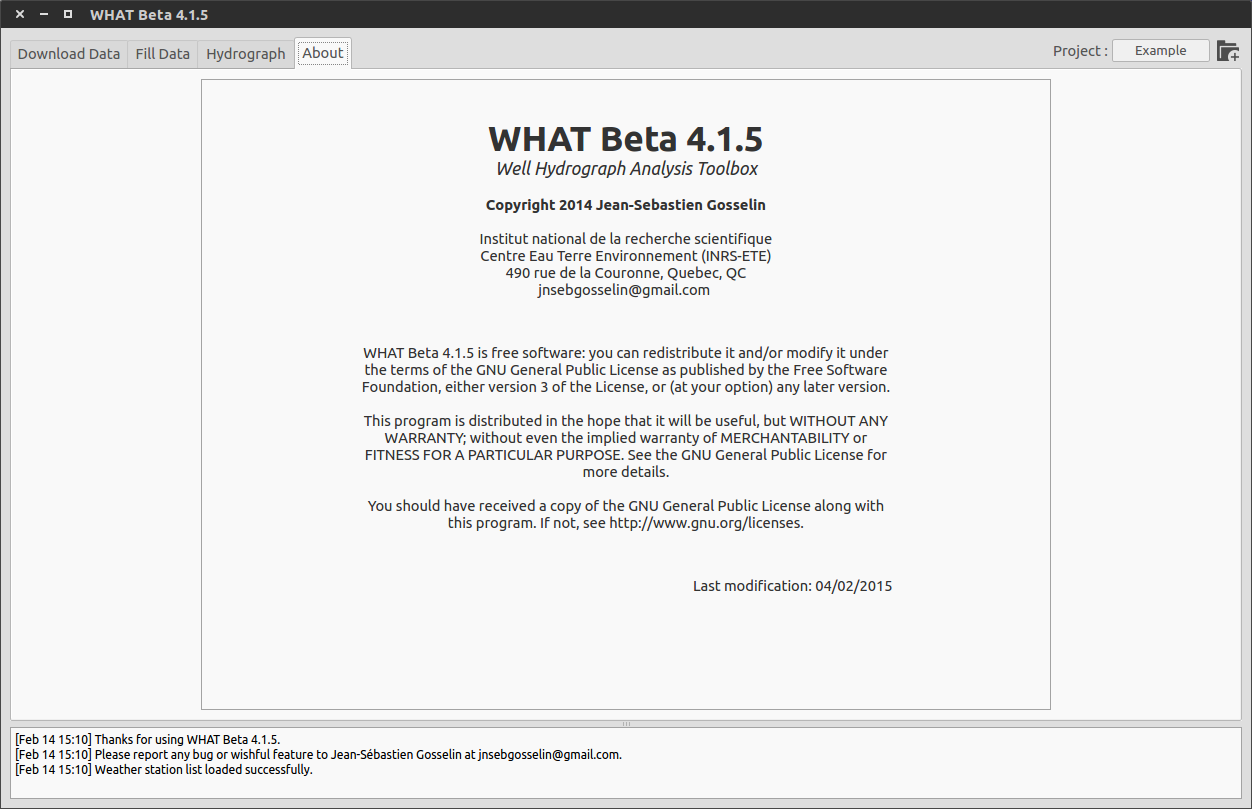
\includegraphics[width=0.75\textwidth]{WHAT_GUI}
\caption[WHAT GUI main features.]{WHAT GUI main features.}
\label{fig:WHAT_GUI}
\end{figure}

\paragraph{Download Data} This tab (see Figure~\ref{subfig:ScnShot_000}) provides an interface to the online Canadian Daily Climate Database (CDCD) that allows to query stations interactively by location coordinates, download the available data, and automatically rearranged the data in a format compatible with WHAT. Alternately, it is possible to provide a custom list of Canadian weather stations for which data can be downloaded and formatted. At the moment, it is not possible to access data of weather stations located in the U.S. This feature may be added in a future release of the software.

\paragraph{Fill} This tab (see Figure~\ref{subfig:ScnShot_001}) is where you can automatically estimate the missing daily weather values in your data to create gapless time-series of daily precipitation and air temperature. Missing data for a given station are estimated from selected neighboring weather stations using a multiple linear regression model.

\paragraph{Hydrograph} This tab is used for viewing and plotting data. For this purpose, two modes are available: the \emph{layout} and the \emph{computation} mode. Both modes share the same weather and water level dataset and it is possible to switch from one mode to the other at anytime. The \textbf{layout} mode (see Figure~\ref{subfig:ScnShot_002}) provides an interface to interactively produce publication-quality graphs from the data. The \textbf{computation} mode (see Figure~\ref{subfig:ScnShot_003}) consists in a dynamic graphical environment where data can be explored, manipulated and analyzed. Various computational tools are available in this mode, including the estimation of the hydrograph Master Recession Curve (MRC) and the estimation of groundwater recharge.

\paragraph{About} This tab (see Figure~\ref{fig:WHAT_GUI}) displays copyright, licensing and general information about WHAT.

\begin{figure}[h!]
        \centering
        \begin{subfigure}[t]{0.45\textwidth}
                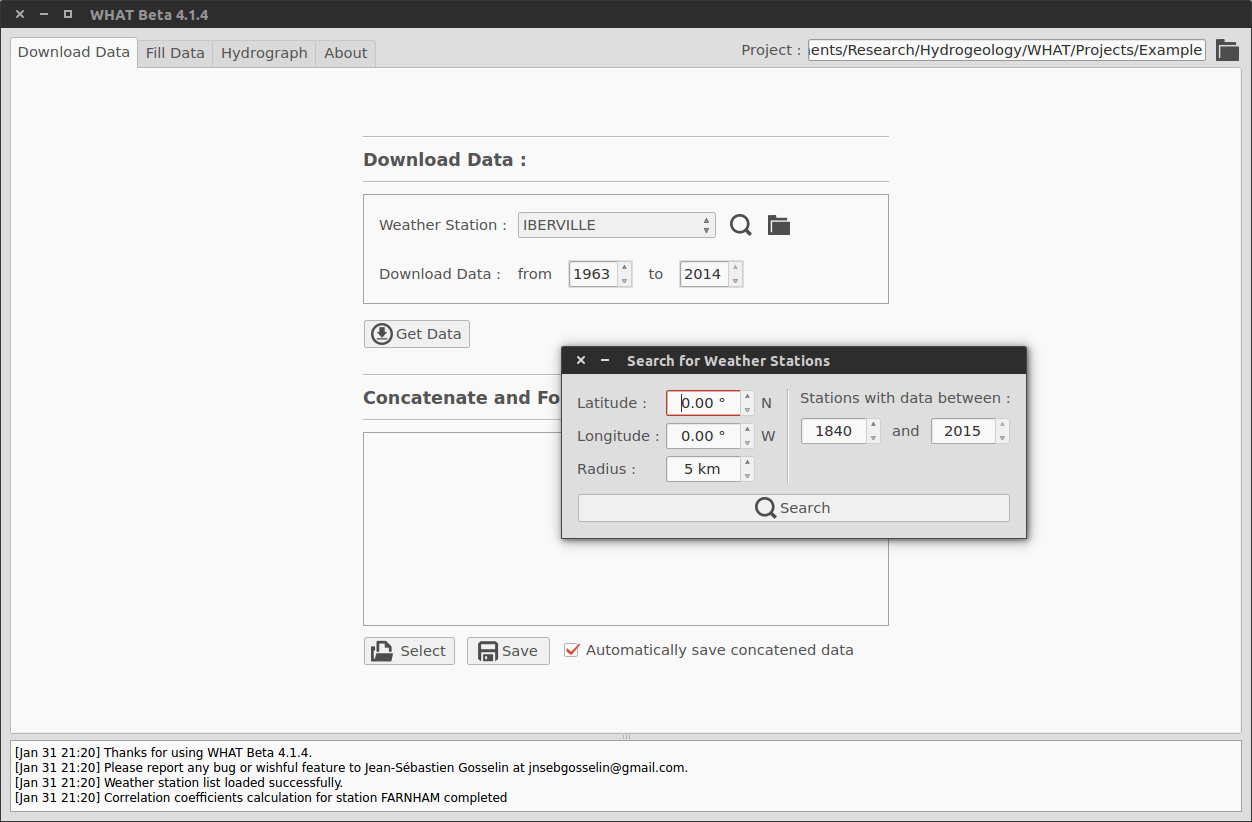
\includegraphics[width=\textwidth]{WHAT_Screenshot000}
                \caption{``Download Data'' tab.}
                \label{subfig:ScnShot_000}                
        \end{subfigure}%
        \hspace{0.5cm}
        \begin{subfigure}[t]{0.45\textwidth}
                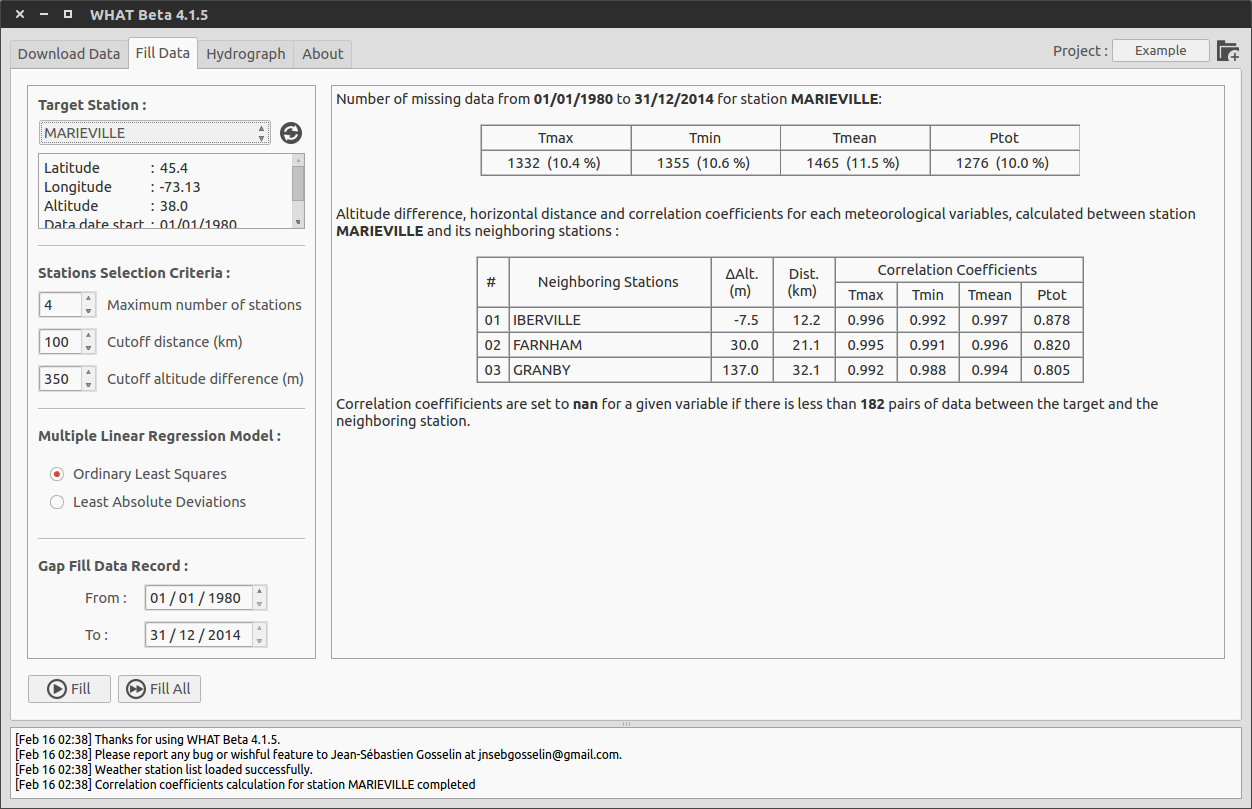
\includegraphics[width=\textwidth]{WHAT_Screenshot001}
                \caption{``Fill'' Data tab.}
                \label{subfig:ScnShot_001}
        \end{subfigure}
        \\[0.5cm]
        \begin{subfigure}[t]{0.45\textwidth}
                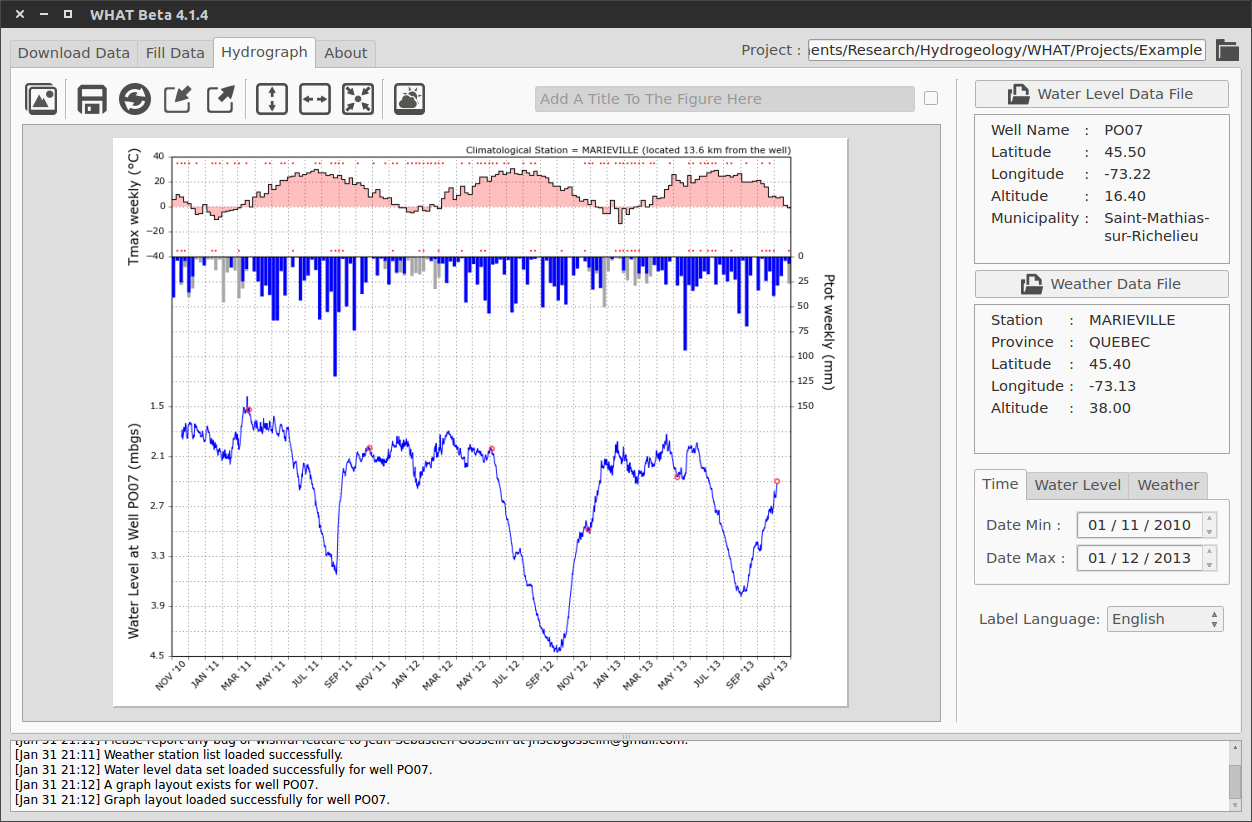
\includegraphics[width=\textwidth]{WHAT_Screenshot002}
                \caption{``Hydrograph'' tab in mode ``Layout''.}
                \label{subfig:ScnShot_002}
        \end{subfigure}
        \hspace{0.5cm}
        \begin{subfigure}[t]{0.45\textwidth}
                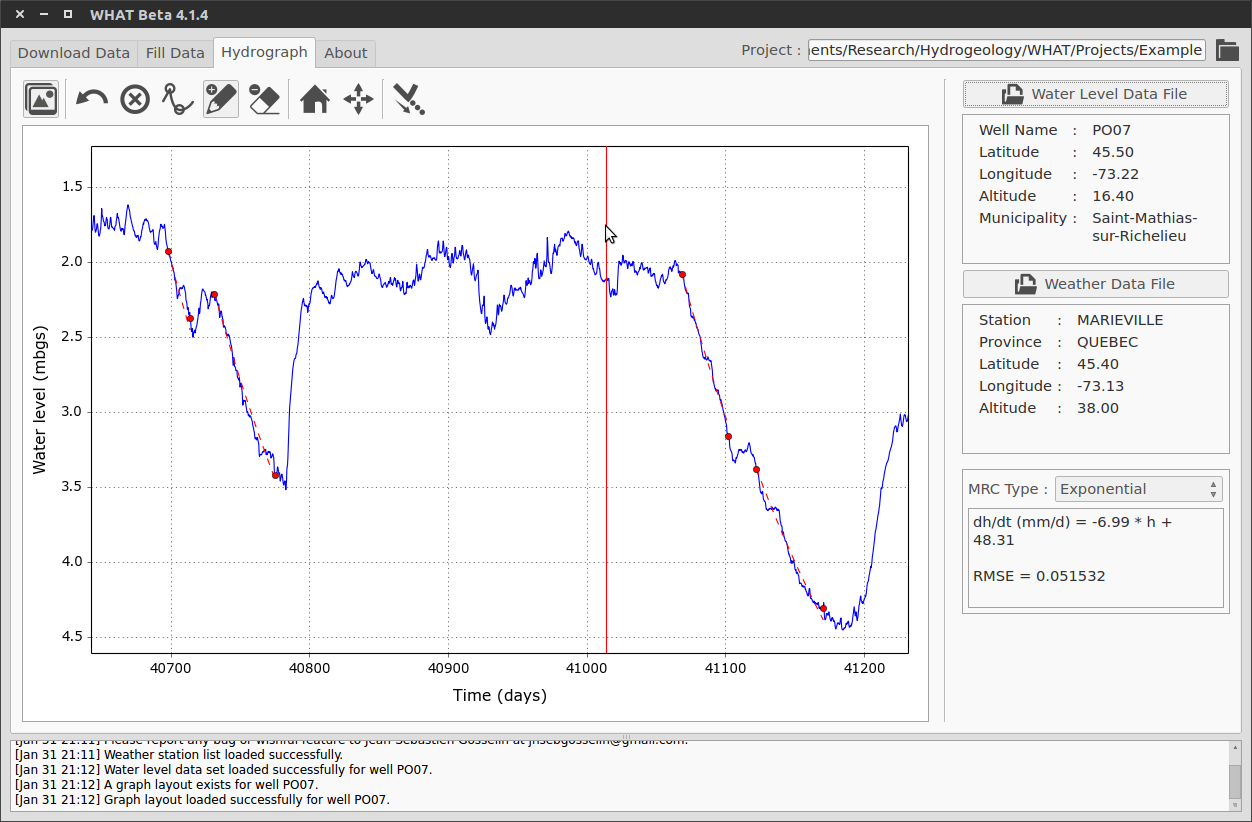
\includegraphics[width=\textwidth]{WHAT_Screenshot003}
                \caption{``Hydrograph'' tab in mode ``Computation''.}
                \label{subfig:ScnShot_003}
        \end{subfigure}
        \caption[Screenshots of WHAT GUI tabs captured in Ubuntu Linux 14.04.]{Screenshot of WHAT GUI tabs captured in Ubuntu Linux 14.04. (a) ``Download Data'' tab. (b) ``Fill'' Data tab (c) ``Hydrograph'' tab in mode ``Layout''. (d) ``Hydrograph'' tab in mode ``Computation''.}\label{fig:WHAT_GUI_ScnShot}
\end{figure}

\section{Workflow for Interpreting Water-level Time-series}

WHAT essentially consists of set of tools to assist the interpretation of water level time series measured in observation wells, from the preparation of raw data to the assessment of groundwater recharge when in unconfined conditions. In this perspective, WHAT was developed with the general workflow shown in Figure 6  in mind.

\begin{figure}[h!]
\centering
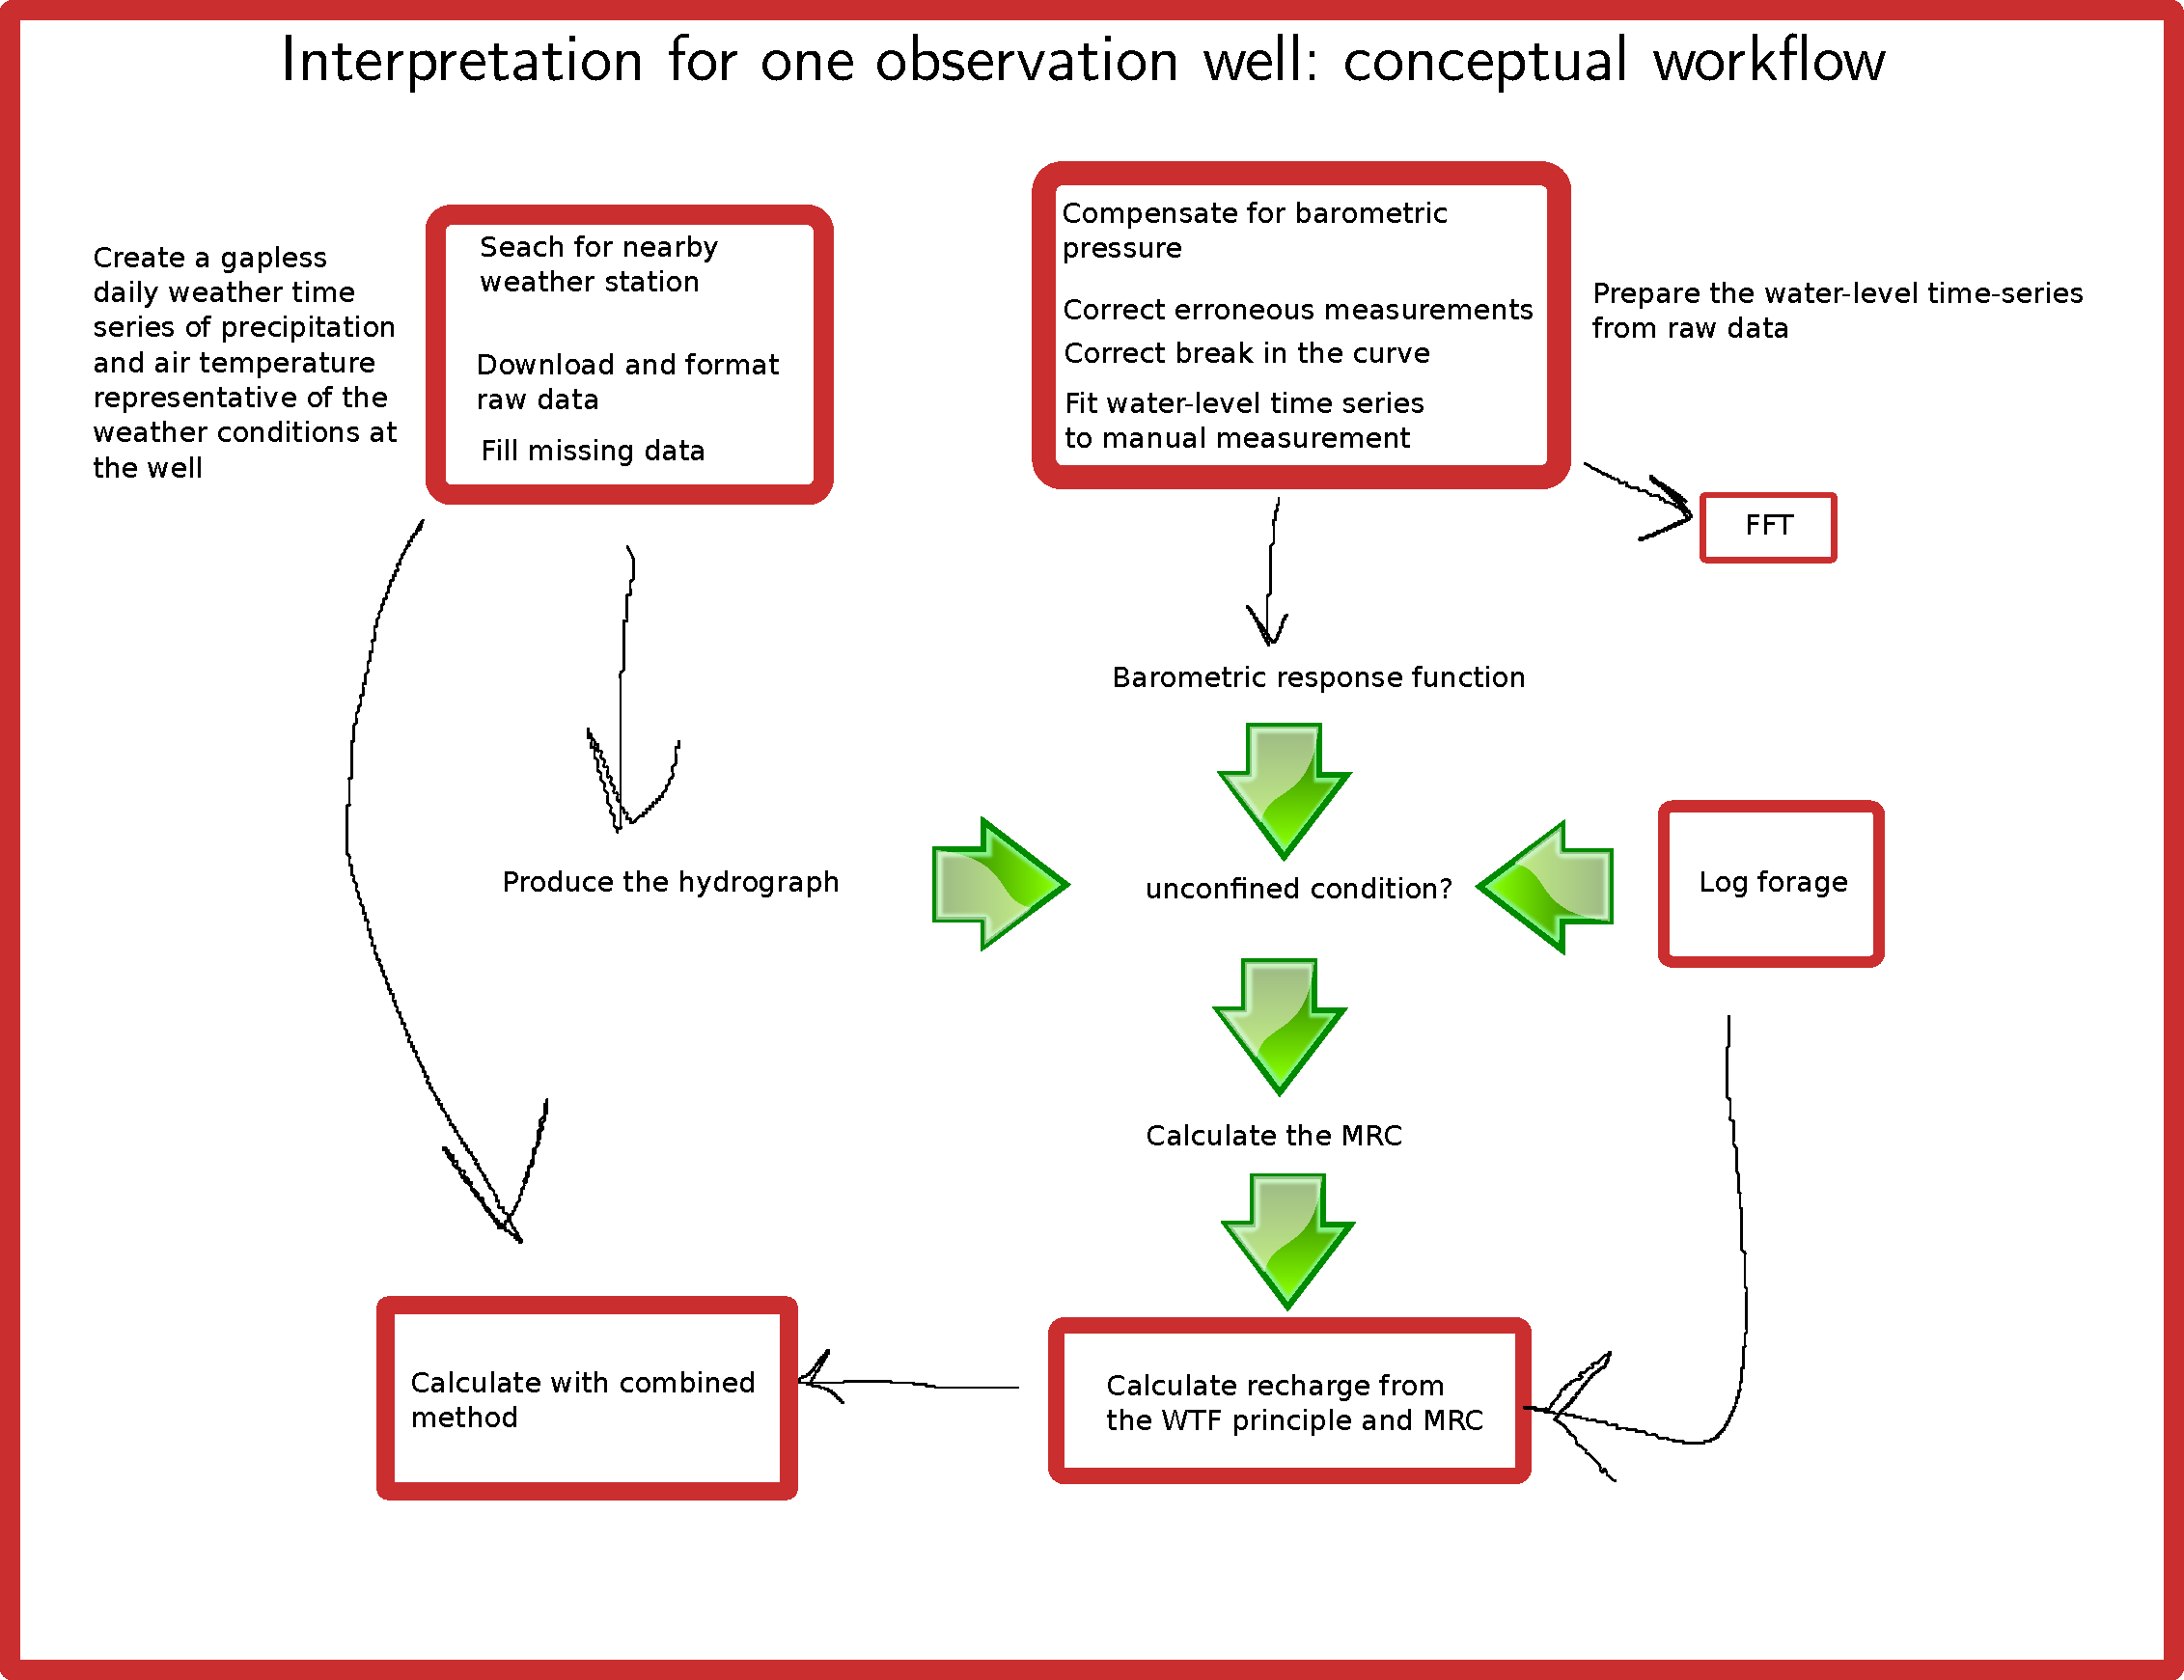
\includegraphics[width=0.95\textwidth]{WHAT_Workflow}
\caption[WHAT conceptual workflow.]{WHAT conceptual workflow for the interpretation of water-level time-series measured in an observation well.}
\label{fig:WHAT_workflow}
\end{figure}

The first step consists in the preparation of a gapless weather dataset.

Validation/preparation of water level time series: 1) automatic measurements fitted to manual measurements. 2) Correct the places where there is a break in the water level curve. This is due generally to the logger that is placed at a different level following the removal of the later from the well. 3) Remove measurements that were acquired while the barologger was outside the water column.

Preparation of a gapless weather dataset. This include. Downloading data from the CDCD database for stations located in a radius of 0 to 100 km from the well. Fill missing daily data for the station located closest to the well by using selected neighboring stations. Data are not interpolated to the exact location of the well. It has been decided to keep the original dataset of the station located closest to the well to analyse the data. This is due to the fact that conventional technique for interpoloating weather data tend to surestimate the number of wet day, but underestimate the intensity of stron precipitation event. More advanced and complicated technique are required to circumvent these issues. It has thus been decided that is was prefereable to keep the original data from a single station.

Once the weather data, and water level are prepared, production of a well hydrograph. Visual interpretation between the water level  fluctuation and weather data can be done.

If high time resolution measurement of the water level and barometric pressure are available, it is possible to carry an calculation of the barometric response function. It is also good to produce a FFT analysis of the hydrograph.
Weather yearly average and montlhy averages can be plotted at this stage.
If the visual inspection of the well, and the barometric response function, determined that the well in unconfined, it means groundwater recharge can be estimated from the data. First, determining the segment where groundwater recharge can be supposed to be negligible and where the water level recede. After that, compute the MRC, and compute a first estimation of groundwater recharge using the Water-Table Fluctuation principle. Estimate finaly recharge with a method combining the meteorological data and the well hydrograph. Enjoy.

\section{Projects Management in WHAT}

\subsection{Introduction}

Data is managed in WHAT by project. That is all input and output files relative to a given project are saved within a common folder called the ``project folder''. This file management system allows you to easily backup and move your projects from one location to the other since all the files relating to a given project are saved at the same place. 

On first launch, WHAT will automatically open an example that is distributed with the software with all the necessary files to easily and quickly test the functionality of the program. The title of the currently opened project is shown in the menu bar at the top of the interface. Additional information about the project can be displayed by clicking on the small ``i'' icon located next to the project name. There can be only one opened project at a time per instance of WHAT. 

\subsection{Create a New Project}

To start a new project, click on the button \textsl{New Project\dots} with the small folder icon located at the right end of the WHAT menu bar (see Figure~\ref{fig:WHAT_GUI}). This will open a new dialog window (see Figure~\ref{fig:new_proj_win}) where you can enter various information about your project such as its title, author and location coordinates. 

Clicking on the button \textsl{Save} creates a new project folder named after your project title in which your project information are saved in a file with a ``.what'' extension. The new folder is created in the location defined by the \textsl{Save in Folder} directory path. For example, saving the \textsl{My New Project} of Figure~\ref{fig:new_proj_win} would create a folder named ``My New Project'' in the directory ``\textsl{C:\textbackslash{}Users\textbackslash{}johndoe\textbackslash{}WHAT\_4.0.5-beta\textbackslash{}Projects}'' and would saved the project information in the file named ``my\_new\_project.what''. It is possible to change the directory where the project folder is created by clicking the small folder icon located next to the \textsl{Save in Folder} directory path.

\begin{figure}[h!]
\centering
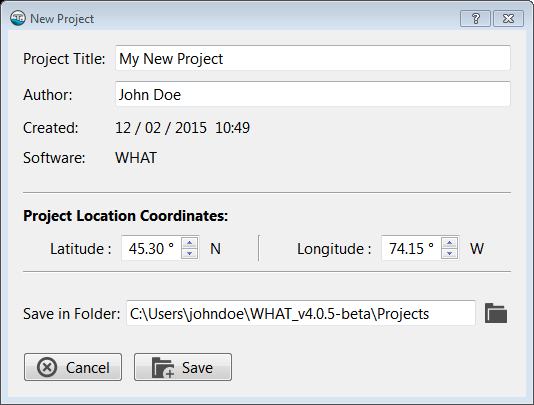
\includegraphics[width=0.5\textwidth]{WHAT_Screenshot_newproject}
\caption[New Project dialog window.]{New Project dialog window.}
\label{fig:new_proj_win}
\end{figure}

\FloatBarrier

\subsection{Open a Project}

To open a new project, click on the name of the currently opened project in the menu bar at the top of WHAT window. This will open a new dialog window where you can browse your folders to select an already existing project file (*.what), and then click Open. WHAT will then open the project and the currently opened project displayed in the menu bar should change to the name of the project you just selected.

The path to your project folder is stored in WHAT in a relative format. This means that if you change the location of your project folder relative the ``WHAT.exe'', your will have to redirect WHAT to the new location of your project by repeating the procedure described in the paragraph above.

\subsection{Project Folder Structure Overview}\label{subsec:folder_structure}

In addition to the project file (.what file extension) that is created when saving a new project, WHAT automatically generates various files and sub-folders that are required for it to run. This file organization is briefly described here and an example is presented in Figure~\ref{fig:proFolder_organization}. The project folder contains two sub-folders named ``Meteo'' and ``Waterlvl'' in addition to a few other files.

\begin{figure}[h!]
\centering
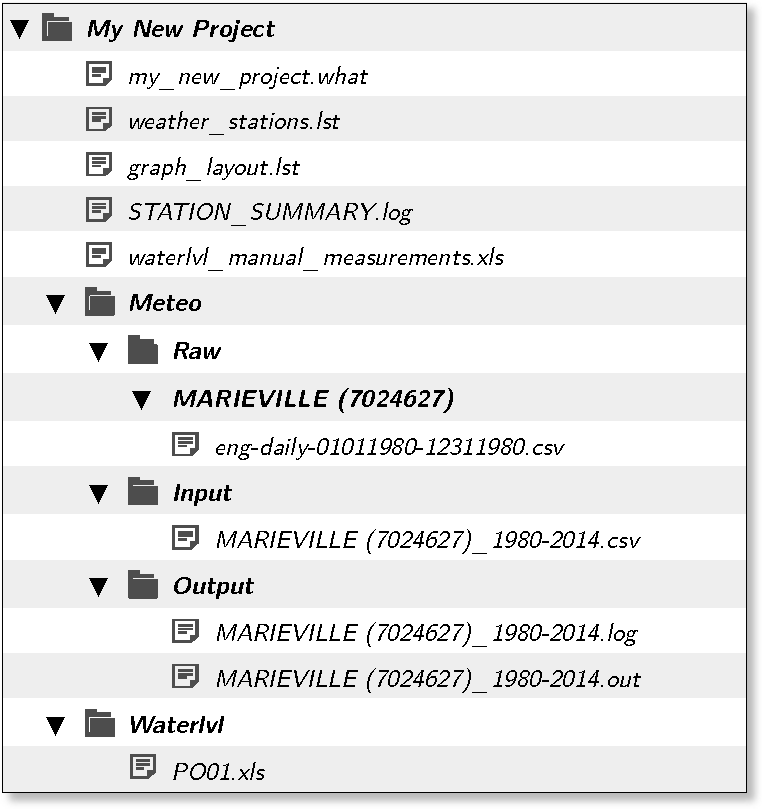
\includegraphics[width=0.5\textwidth]{file_and_folder_architecture}
\caption[Project folder file organization.]{Project folder file organization.}
\label{fig:proFolder_organization}
\end{figure}

\paragraph{Meteo} The folder \emph{Meteo} contains three sub-folders named respectively Raw, Input and Output. The folder \textbf{Raw} is where are saved the weather data files downloaded from the CDCD. These are coma-separated values (CSV) files that contain weather data on a yearly basis. All the data files for a given weather station are saved within a common folder named after the station name and its unique identification number (IDN). For example, in Figure~\ref{fig:proFolder_organization}, the raw data file ``eng-daily-01011980-12311980.csv'' that contains weather data of the station ``Marieville'' for the year 1980 is saved within a folder named ``MARIEVILLE (7024627)'' where the number in parentheses is the unique IDN of the station.

The folder \textbf{Input} contains the formatted weather data files produced from the raw data files. These are tab-separated values (TSV) files that are named after the station's name and IDN.

The folder \textbf{Output} is where are saved the gapless weather time-series produced from the content of the Input folder. These are saved in TSV text files with the extension ``.out''. The files with the extension ``.log'' are TSV text files that contain detailed information about every missing daily weather value that were estimated by the program to produce the gapless time-series (.out files).

\paragraph{Waterlvl} The folder ``Waterlvl'' is the preferred location were your water level time-series should be stored. These files can be  either in a Microsoft Excel spreadsheet file format (xls) or in a tab-separated values text format (TSV).

\paragraph{Other Files}The file ``weather\_stations.lst'' is a resource file that is used to store the results of a weather station search in the Canadian Daily Climate Database (CDCD). The file ``graph\_layout.lst'' is also a resource file in which are stored the layout parameters of the well hydrographs that are produced in the hyhdrograph tab of WHAT. The file ``STATION\_SUMMARY.log'' is an tab-separated values (TSV) file that contains a summary of all the weather data files contained in the ``Input'' folder. The file ``waterlvl\_manual\_measurements.xls'' is used to input manual water level measurements associated with the water level time-series files stored in the ``Waterlvl'' folder. These measurements are plotted on the hydrograph and can also be used to adjust the position of the water-level time-series in the vertical axis when the installation depth of the pressure probe is unknown.

\FloatBarrier

\section{Creation of gapless weather data series}

\subsection{Downloading and formatting data from the CDCD database}

\begin{figure}[h!]
\centering
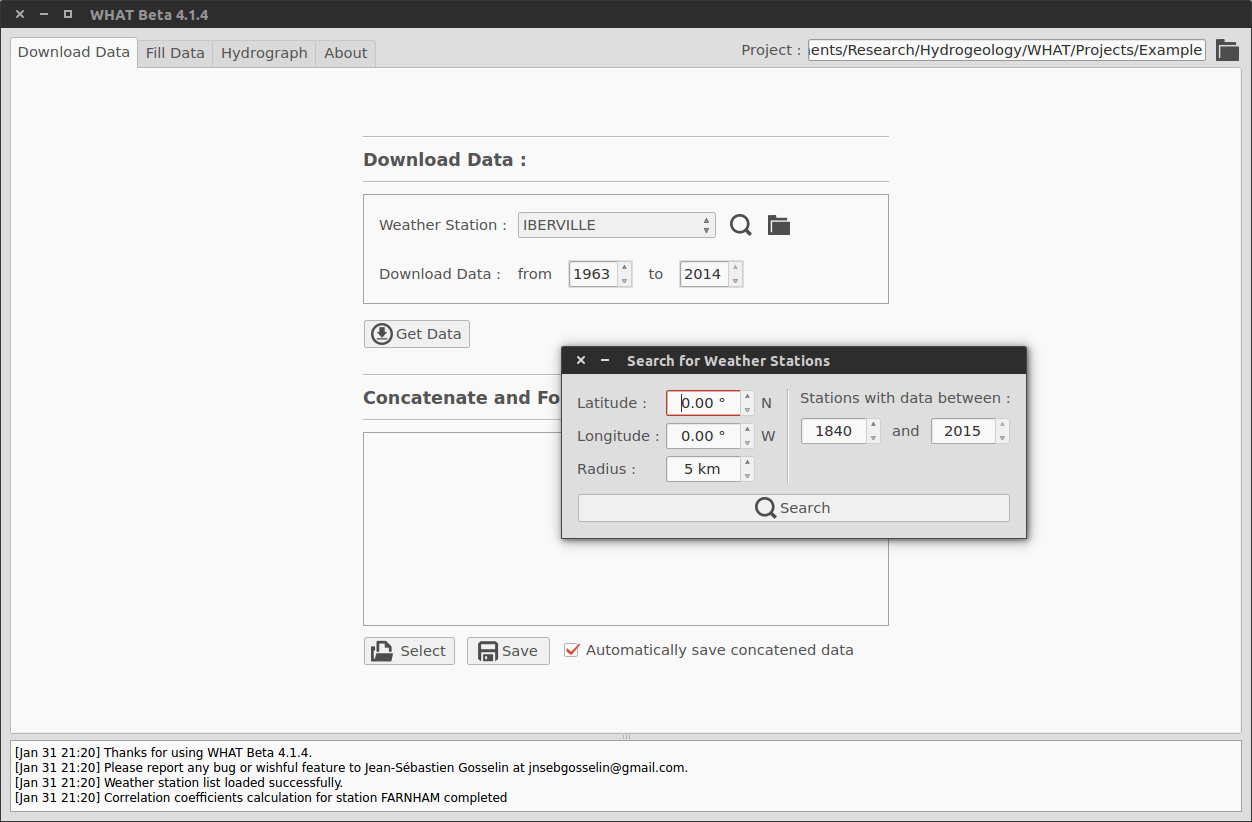
\includegraphics[width=0.75\textwidth]{WHAT_Screenshot000}
\caption[Tab ``Download Data''.]{Tab ``Download Data''.}
\label{fig:tab_dwnldData}
\end{figure}

The Canadian Daily Climate Database (CDCD) contains daily air temperature and precipitation from 1840 to the present for about 8450 stations distributed across Canada. Data can be downloaded manually on the Government of Canada website as CSV files on a yearly basis, or it is possible to acquire the entire database by ordering a DVD. The former option involves a lot of repetitive manipulations and can become quickly a time consuming task while the latter does not offer a convenient way to update your data. Moreover, the organization of the original CDCD data files in a more convenient format can also represent a tedious task when done manually. WHAT alleviates this process by providing a graphical interface to the online CDCD database that allows to query stations interactively by location coordinates, download the available data, and automatically rearranged the data in a format compatible with WHAT. All of these features are available from the tab \emph{Download Data} shown in Figure~\ref{fig:tab_dwnldData}.

\subsubsection{Searching for Stations}

To start searching for stations in the online CDCD, go in the tab \emph{Download Data} and click on the small magnifying glass icon located next to the \emph{Weather Station} drop down list, that should be empty if you have just created a new project. This will open a new dialog window (see Figure~\ref{fig:Screenshot_search4stations}) where you can search for stations located within a given radius around a location defined in latitude and longitute decimal degrees. It is possible to further narrow down the search by including only stations that have data within a given period. 

Clicking on the button \emph{Search} initiates the search for weather stations with the specified parameters. The results are saved in the file ```weather\_stations.lst'' and the \emph{Weather Station} drop down list is updated to list all the stations found during the search.

\begin{figure}[h]
\centering
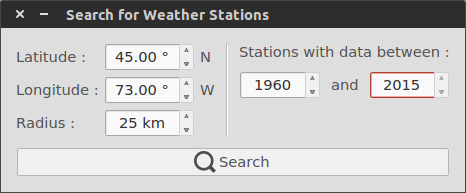
\includegraphics[width=0.5\textwidth]{WHAT_Screenshot_search4stations}
\caption[Graphical interface to the online CDCD database.]{Graphical interface to the online CDCD database.}
\label{fig:Screenshot_search4stations}
\end{figure}

Alternately, it is possible to use a custom list of Canadian stations generated manually without using the graphical interface. This is done by retrieving station information from their unique url directly on the government of Canada website (\url{www.climate.weather.gc.ca}). The information must be saved in a TSV text file with the ``.lst'' extension. The list can be loaded in WHAT by clicking on the small folder icon located next to the \emph{Weather Station} drop down list. A detailed example is presented for the weather station Marieville, located in southern Quebec, in Appendix~\ref{app:custom_station_list}.

\subsubsection{Downloading Data}

Once a list of weather station has been generated in WHAT, either by an automatic search with the interface or by opening a custom weather station list, data can be downloaded from the online CDCD by selecting the desired station in the drop-down menu list and clicking on the button \emph{Get Data}. For each year between the values specified in the \emph{Download Data} year range, WHAT will automatically download the weather data from the CDCD and save the results as a CSV file in the \emph{Raw} folder (see section~\ref{subsec:folder_structure} for each year individually).

The downloading process can be stopped at any time by clicking on the button \emph{Get Data} which will then be displaying a red stop icon. Before downloading data for a given year, WHAT will first check if data already exist for that whole year in the folder \emph{Raw}. If it is the case, data for this year won't be downloaded and the process will pass to the following year, otherwise data will be downloaded and saved normally from the CDCD. Detailed information about the program transactions during the downloading process are printed in the console area located at the bottom of the interface (see section~\ref{sec:GUI_overview}).

\subsubsection{Formatting Data}

As soon as a downloading task ends successfully for a given weather stations, WHAT automatically format and concatenate the data. That is data for each year are put together end to end in chronological order and only data related to air temperature (mean, max and min) and total precipitation are kept. In addition, NaN values will be put everywhere data are missing. Finally, statistics about the missing values in the dataset for each meteorological variable will be displayed in the \emph{Concatenate and Format Raw Data Files} section.

By default, WHAT will automatically save the formatted data series in a single TSV file within the folder \emph{Input} (see section~\ref{subsec:folder_structure}. You can save any other copy of the formatted data set anywhere on your computer by clicking on the button \emph{Save}. The automatic saving of formatted data series can be disabled by unchecking the \emph{Automatically save concatenated data} option. 

It is also possible to open previously downloaded weather data files in WHAT by clicking on the button \emph{Load} and selecting the desired files in the dialog window. WHAT will then automatically format and concatenate the data and a new concatenated data files and save the results automatically if the \emph{Automatically save concatenated data} option is checked. Alternatively, the formatted data series can be saved by clicking on the button \emph{Save}.

\subsection{Gap filling daily weather records}

One of WHAT main utility is the automatic gap filling of daily weather data records. This feature is accessible from the tab \emph{Fill Data} shown in Figure~\ref{fig:tab_fillData}. On start-up or after opening a project, WHAT automatically scans the content of the \emph{Input} folder for valid weather data files and displays the result as a list of weather station names under the label \emph{Fill Data for Weather Station}. The list of stations won't be refreshed automatically if new data files are added to the Input folder after the project has been opened. The button \emph{Refresh} located next to the list of stations can be used for this purpose. In addition, each time WHAT search the Input folder for valid weather data files, it automatically computes statistics about the period over which data are available for each station and the number of missing data in the weather time-series and saves the results in the file named ``STATION\_SUMMARY.log'' (see section~\ref{subsec:folder_structure}).

\begin{figure}[h!]
\centering
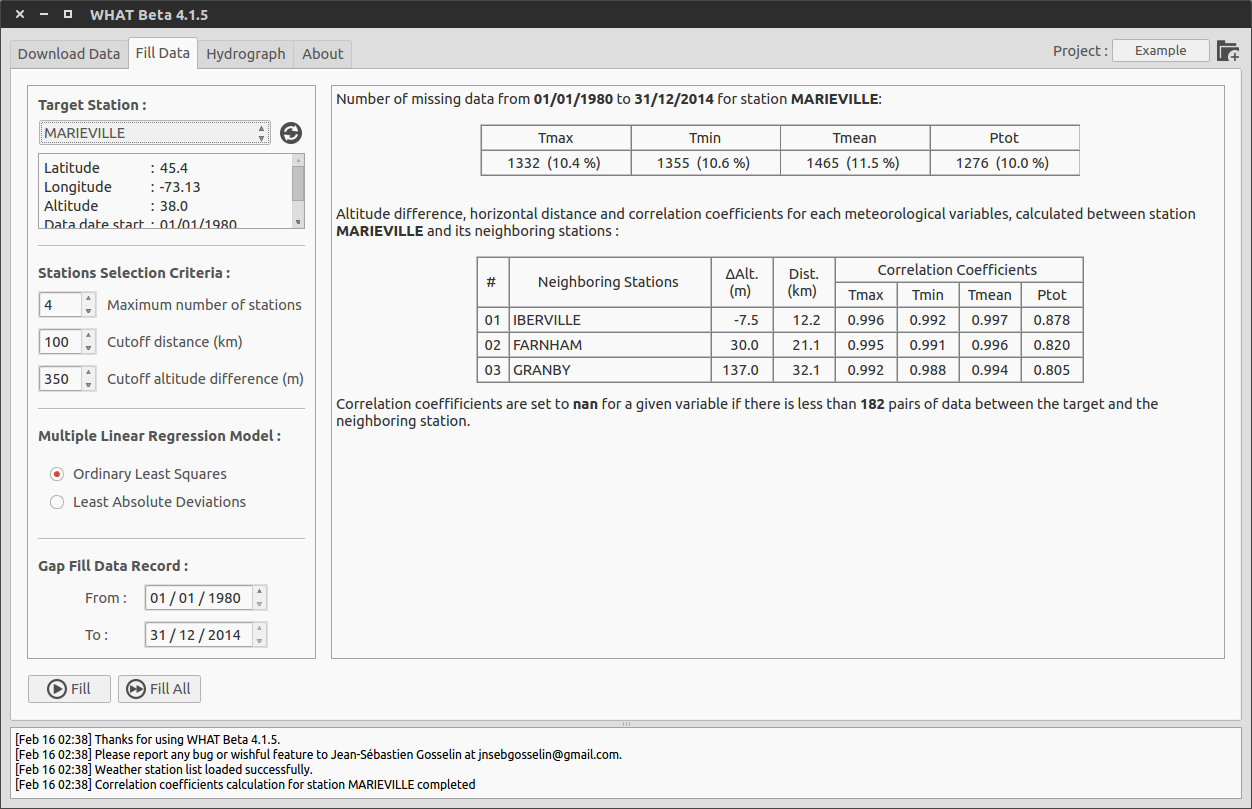
\includegraphics[width=0.75\textwidth]{WHAT_Screenshot001}
\caption[Tab ``Fill Data''.]{Tab ``Fill Data''.}
\label{fig:tab_fillData}
\end{figure}

If the Input folder is not empty, selecting a station from the drop-down list will automatically initiate the computation of correlation coefficients between the data of the selected station and all of the remaining stations (herein called the neighboring stations), as well as horizontal distances and elevation differences. In addition, information about the number of missing values in the data of the selected weather station are also computed. The results are displayed in the view panel located on the right side of the interface. Correlation coefficients that fall below a value of 0.7 are displayed in red in the table. This is only meant as guidance for the user and has no impact on the gap filling procedure.

The process to fill the gaps in the data of the selected weather station can be launched by clicking the button \emph{Fill} located at the bottom of the left side panel of the interface. Each missing value is estimated with a multiple linear regression (MLR) model generated with the synchronous weather time series of the selected and neighboring stations. The routine uses the data from the neighboring stations that are best correlated with the data of the selected station, up to the maximum number of stations defined by the user. For example, in Figure~\ref{fig:tab_fillData}, the program would use the neighboring stations with the best correlation coefficient values up to a maximum of 4 stations. If for a given date all the neighboring stations have missing data synchronously with the selected station, a NaN value is kept in the dataset at this particular time.  

It has been demonstrated that the MLR method outperforms most of the commonly used techniques for the estimation of missing data in daily meteorological records \citep{eischeid_quality_1995,eischeid_creating_2000,xia_forest_1999}. The user can also choose between an Ordinary Least Squares (OLS) or a Least Absolute Deviations (LAD) criterion for the generation of the MLR model. The LAD criteria is more robust to outliers than the OLS but is more demanding in computation time. 

In addition, data correlation between two stations for a given meteorological variable will generally decreases as difference in altitude and distance increase. Therefore, it is possible to specify a cutoff distance and a cutoff altitude difference for which neighboring stations that fall above these cutoff values are excluded from the gap filling procedure. A value of 100~km for the cutoff distance and 350~m for the cutoff altitude difference are set as default values in the program, based on the literature 
\citep{tronci_comparison_1986,xia_forest_1999,simolo_improving_2010}. 

WHAT will fill the gaps in the data between the dates specified by the user and automatically save the gapless daily weather time series in a tab-separated values (TSV) text file with the extension ``.out'' within the sub-folder \emph{Output} of the folder \emph{Meteo} (see section~\ref{subsec:folder_structure}). The file is named after the weather station name and its unique IDN. For example, the resulting output file for the station named Marieville in Figure~\ref{fig:tab_fillData} would be ``MARIEVILLE (7024627)\_1980-2014.log''. In addition, detailed information about every missing value estimated by WHAT to fill the gap in the data are saved in a file with the same name as the ``.out"" file but with a ``.log'' extension.

It is also possible to fill the gaps in the data for all the stations in batch by clicking on the button \emph{Fill All}. The parameters for the gap filling process will then be kept the same for all the stations.

Finally, it is possible to assess the incertitude of the method used to estimate the missing values with a jackknife procedure. However, this is an experimental feature that is not presently available from the GUI and must be activated directly in the source code.

\subsection{Use of weather data from other sources}

Presently, it is not possible to access data of weather stations located in the U.S. or in any other contry than Canada. This feature may be added for the U.S. in a future release of the software however.

Nevertheless, it is still possible to use weather data from any sources in WHAT for the gap filling procedure or the interpretation of water-level time-series, as long as the data are saved in a format compatible with WHAT.

Samples of input and output files are provided in the example project folder that is distributed with the software. Data must be saved in a tab-separated values text file with the extension.csv if 

be tab-separated and saved in a file with a csv extension. This can be easily achieved in any standard spreadsheet application such as Microsoft Excel or LibreOffice Calc. The format of the header must be observed faithfully (see example in Figure 1). NaN values must be inputted where data are missing. Data must also be in chronological order, but do not need to be continuous over time. That is missing blocks of data (e.g., several months or years) can be completely omitted in the concatenated data file. These missing blocks of data will be estimated and filled during the gap filling procedure.

\section{Preparation of the water level time series}

\subsection{Data validation and correction}

Pour chacun des puits, les valeurs de niveaux d’eau obtenues avec les sondes ont été comparées avec des mesures manuelles prises lors des visites aux puits. Pour l’ensemble des puits, l’écart absolu entre les valeurs des sondes et les mesures manuelles est généralement inférieur à 5 cm.

Pour un même puits, lorsqu'un écart systématique de plus de 5 cm était observé entre les mesures manuelles et les mesures automatiques, une correction des niveaux d’eau a été  appliquée de façon à caler les valeurs obtenues avec les sondes aux mesures manuelles.
Les données aberrantes dans les séries de données ont également été corrigées par interpolation linéaire. C’est données aberrantes sont principalement des mesures qui ont été prises alors que la sonde avait été retirée du puits pour le téléchargement des données, ou encore par du pompage dans les puits lors d’une campagne d’échantillonnage de l’eau.

\subsection{Generation of the well hydrograph with weather data}

The view can be panned by dragging the mouse with the left mouse button depressed. Zoom in by pressing the Ctrl key while dragging the mouse upwards, or by moving the mouse wheel up. Zoom out mouse wheel down.

\subsection{Barometric response function}
\subsection{Estimation of the MRC and first recharge estimation}
\subsection{Recharge estimation with synthetic well hydrograph method}

\chapter{Technical Documentation}

\section{Barometric correction: an overview}

\cite{freeman_use_2004}

Even though there exists software that can correct data automatically for barometric pressure, it is always a good practice to understand what is done behie. This is particularly usefull to correct situations when something goes wrong. For example, the barologger may had a deficiency and atmospheric pressure needed to be taken from the CDCD for example and data needed to be corrected manually. There arise often situation when correction needs to be done manually. This happens when there is a problem with the data. This is then good practice to understand the process in order to dodge mistake.

It is a good idea to monitor water level at a 15 min frequency for a period of a year, or more if it is possible. The data can be used subsequently to estimate the barometric response function of the well that can be quite usefull to understand the hydrogeological context, and the level of confinement of the well. Having data with this frequency is also usefull for running FFT and understand the cause of possible unatural fluctuation in the well.

\begin{figure}[h!]
\centering
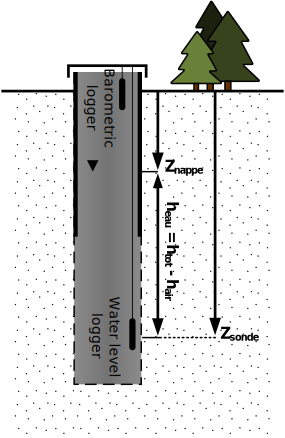
\includegraphics[width=0.5\textwidth]{ObsWell}
\caption[Typical instrument configuration for water level monitoring in an observation well]{Typical instrument configuration for water level monitoring in an observation well}
\label{fig:obswell_config}
\end{figure}

\subsection{Format des données brutes}

Le monitoring des niveaux d’eau dans les puits d’observation pour le projet Montérégie Est a été fait avec des sondes à niveaux d’eau non ventilées. Cela implique que pour pouvoir calculer la hauteur de la colonne d'eau, heau, située au-dessus des sondes (voir figure 1), la pression atmosphérique doit également être connue à chacun des puits. À cet effet, des sondes barométriques ont également été installées dans la majorité des puits d'observation du projet Montérégie Est. Une attention particulière a été portée afin d'assurer que les puits qui n'étaient pas munis d'une sonde barométrique étaient situés à proximité et à une altitude raisonnablement similaire d'un puits où la pression atmosphérique était mesurée.

La profondeur de la nappe par rapport à la surface, Znappe, est calculée via l'équation suivante : 

où Znappe (m) et Zsonde (m) correspondent respectivement à la position de la nappe et la profondeur d'installation de la sonde à niveaux d'eau par rapport à la surface du sol, htot (m) est la charge totale mesurée par la sonde à niveaux d'eau et hatm (m) est la charge mesurée par la sonde barométrique. L'axe des z est défini positif vers le haut avec, pour niveau de référence, la surface du sol. Ainsi Zsonde et Znappe ont des valeurs qui sont généralement inférieures à zéro, à moins que le niveau de l'eau dans le puits ne soit situé au-dessus de la surface.

Au cours du projet, trois modèles de sondes ont été utilisés pour la mesure des niveaux d’eau: (1) levelogger Gold de Solinst, (2) levelogger Edge de Solinst et (3) Micro-Diver de Schlumberger. Parallèlement, deux modèles de sondes ont été utilisés pour la mesure de la pression atmosphérique: (1) barologger Gold de Solinst et (2) barologger Edge de Solinst. Il est important de savoir que la méthode de stockage des données brutes varie d'un instrument à l'autre. C’est-à-dire que des transformations mathématiques sont parfois appliquées sur les mesures avant de les mettre en mémoire. En général, cela ne cause pas de problème car les logiciels de traitement des données fournis par les fabricants gèrent le tout de façon automatique et implicite. Par contre, lorsqu'une manipulation manuelle des données brutes est nécessaire ou lorsque des analyses plus complexes sont envisagées, une connaissance des différentes stratégies de stockage des instruments est essentielle.
Pour les sondes levelogger et barologger Gold, les données brutes enregistrées par les instruments correspondent aux pressions mesurées, converties en hauteur d'eau équivalente, moins une constante dont la valeur est établie en fonction de la pression atmosphérique minimale anticipée au niveau de la mer et de l'altitude fournie à la sonde par l'utilisateur lors de sa programmation (9.5 m - 0.0012 m par mètre d'altitude). Pour les sondes Micro-Diver et Levelogger Edge, les données brutes enregistrées par les instruments correspondent aux pressions mesurées converties en hauteur d'eau équivalente. Enfin, pour les sondes barologger Edge, la pression atmosphérique est directement mise en mémoire sans aucune transformation préalable. Le Tableau 1 résume les différentes opérations mathématiques qui sont appliquées aux mesures avant de les mettre en mémoire pour les différents types de sondes qui furent utilisées au cours du projet Montérégie.

où Ptot (kPa) est la pression absolue ressentie par la sonde à niveaux d'eau, Patm (kPa) est la pression atmosphérique, ρ (kg/m3) est la masse volumique de l'eau, g (m/s2) est l'accélération gravitationnelle terrestre et Zalt (m) est l'altitude du puits fourni à la sonde par l'utilisateur lors de sa programmation.

% \chapter{Code Architecture}

\appendix
\chapter{Creating a Custom CDCD Weather Station List}
\label{app:custom_station_list}

WARNING: this section needs to be updated and revised.

The stations information need to be saved in a tabular-separated values text file with an “lst” extension. A template of a station list (station\_list\_template.lst) is provided with the program in the Zip archive and an example is presented in Error: Reference source not found. The fields Station Name, Year, Start, Year End and Province do not need to match strictly with the station's URL. These fields can be assigned any name/value by the user and are not directly used in the downloading process of weather data. The only field that is directly used in the download process is Station ID that is a unique number attributed to each weather station.

Once a file containing a list of weather stations' information has been created, it is possible to load it in Rainbird by clicking on the  Load button located in the Fetch and Merge tab (Error: Reference source not found). The station list can be refreshed at any time by clicking on the  Refresh button.

\begin{figure}[h!]
\centering
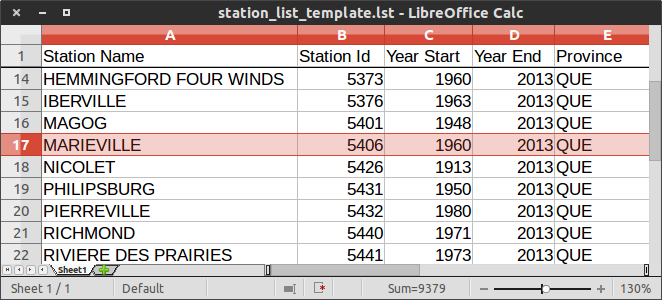
\includegraphics[width=0.5\textwidth]{example_staList}
\caption[Weather Station List (*.lst) Sample]{Weather Station List (*.lst) Sample}
\label{fig:example_staList}
\end{figure}

\paragraph{Step 1} First go to \url{www.climate.weather.gc.ca}.

\paragraph{Step 2} At the bottom of the page, click on Advanced Search (see the red arrow in Figure~\ref{subfig:customWeaterStaList_step1}).

\paragraph{Step 3} Search for a station either by Province, Name or Proximity. For this example, the search was made using the Name of the station (see Figure A2).

\paragraph{Step 4} The research yielded one result (Figure A3). For Data Interval, select Daily and click Go.
	WARNING: The downloading and formatting of Hourly data is not currently supported in Rainbird.

\paragraph{Step 5} The URL associated with Marieville weather station is:\\[0.1cm]

\begin{sloppypar}
\noindent
\url{http://climate.weather.gc.ca/climateData/dailydata_e.html?timeframe=2&Prov=QUE&StationID=5406&dlyRange=1960-06-01|2013-12-31&Year=2013&Month=12&Day=01}.\\[0.1cm]
\end{sloppypar}

From this URL, we find that its Station ID is 5406 (see red circle in Figure A4), that is located in the province of Quebec (QUE) and that data are available from 1960 to 2013.

\begin{figure}[h!]
        \centering
        \begin{subfigure}[t]{0.45\textwidth}
                \centering
                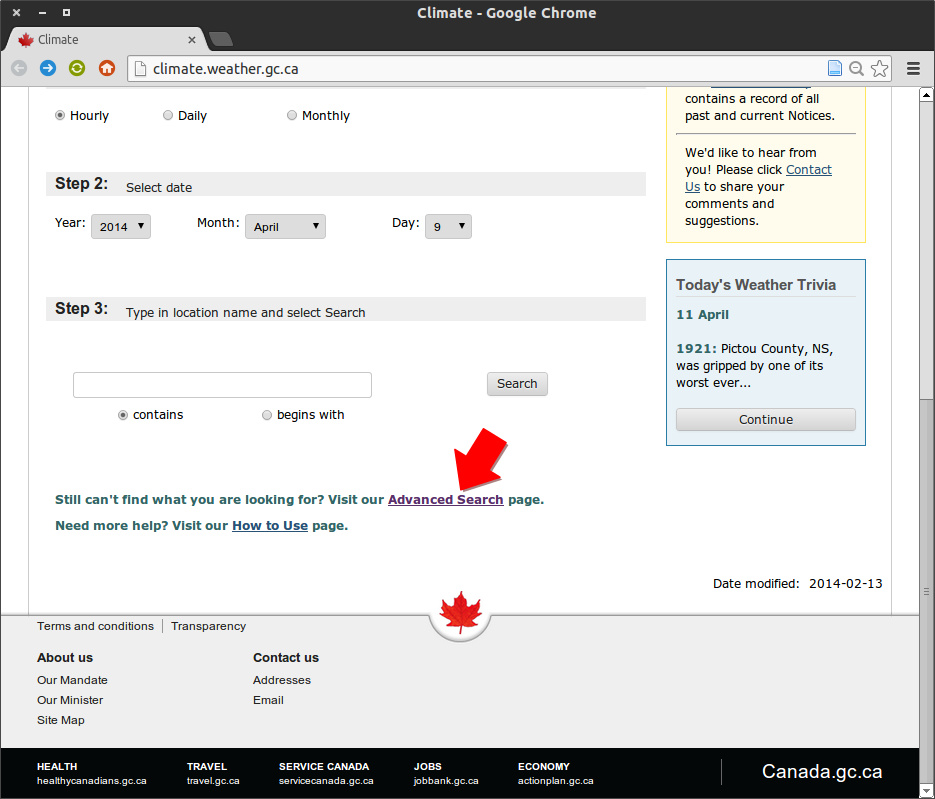
\includegraphics[width=\textwidth]{customWeaterStaList_step1}
                \caption{Step 1}
                \label{subfig:customWeaterStaList_step1}                
        \end{subfigure}%
        \hspace{0.5cm}
        \begin{subfigure}[t]{0.45\textwidth}
                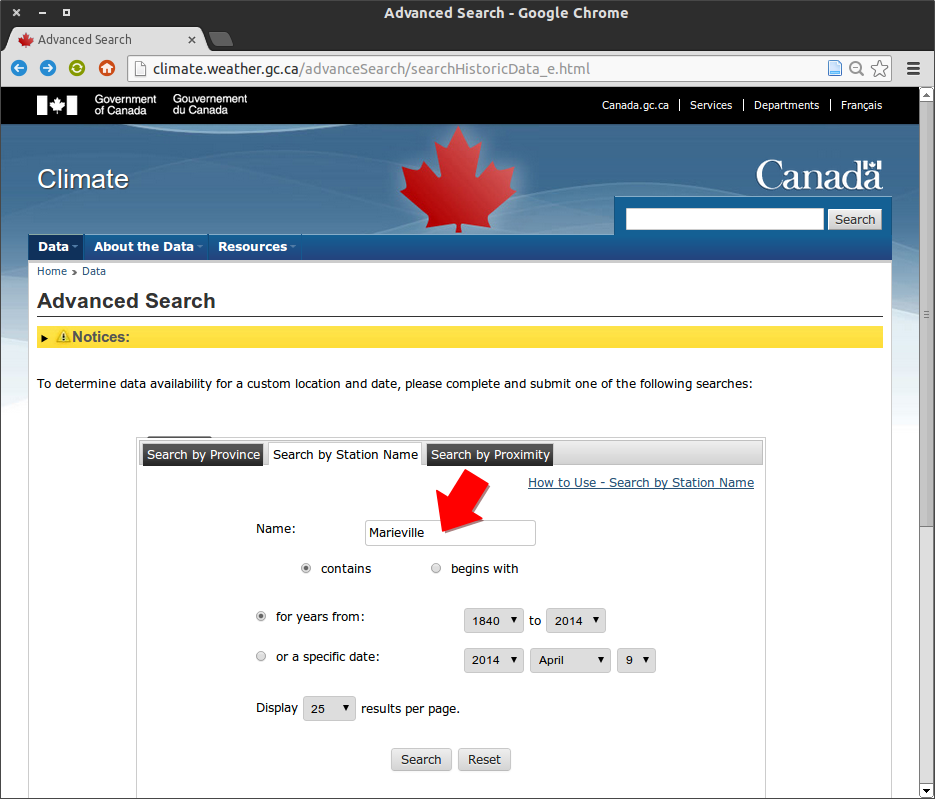
\includegraphics[width=\textwidth]{customWeaterStaList_step2}
                \caption{Step 2}
                \label{subfig:customWeaterStaList_step2}
        \end{subfigure}
        \\[0.5cm]
        \begin{subfigure}[t]{0.45\textwidth}
                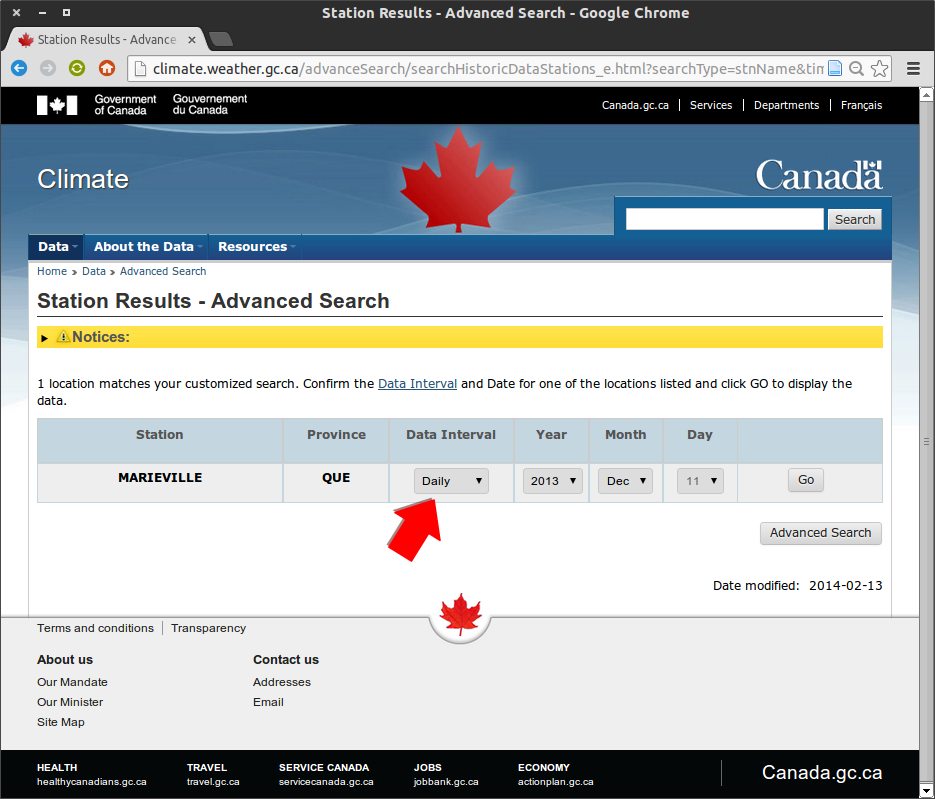
\includegraphics[width=\textwidth]{customWeaterStaList_step3}
                \caption{Step 3}
                \label{subfig:customWeaterStaList_step3}
        \end{subfigure}
        \hspace{0.5cm}
        \begin{subfigure}[t]{0.45\textwidth}
                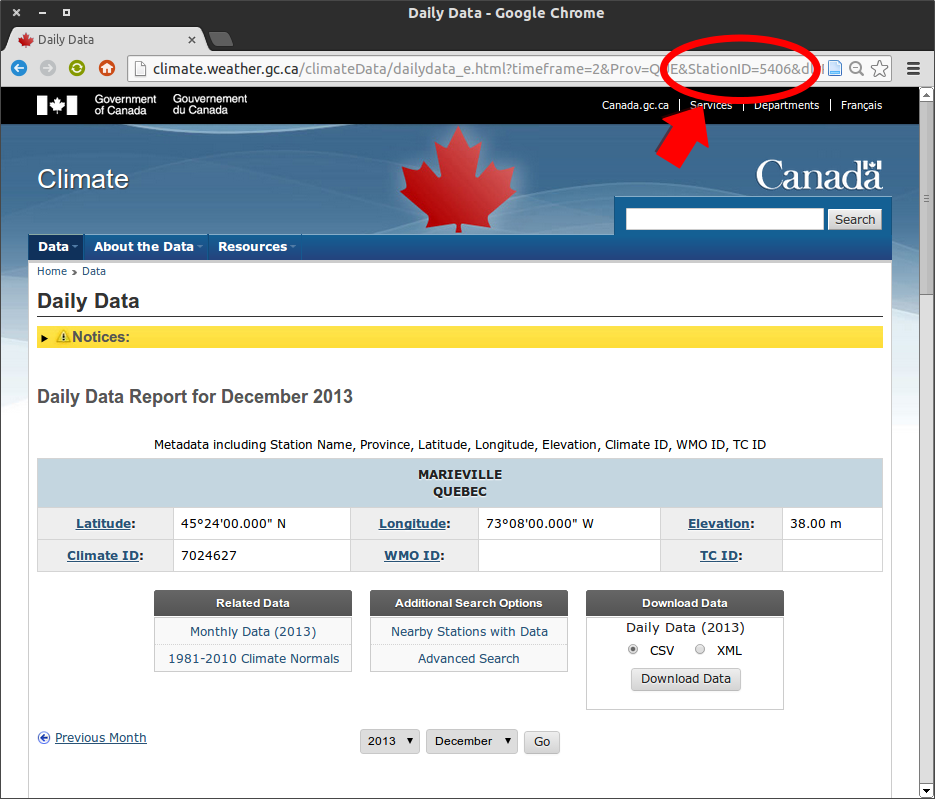
\includegraphics[width=\textwidth]{customWeaterStaList_step4}
                \caption{Step 4}
                \label{subfig:customWeaterStaList_step4}
        \end{subfigure}
        \caption[Creation of a custom weather station list how-to]{Creation of a custom weather station list how-to}\label{fig:customStaList_Howto}
\end{figure}



\bibliography{WHATMANUAL}

\end{document}